\documentclass[border=10pt]{standalone}

\usepackage{tikz}
\usepackage{tikzsymbols}
\usetikzlibrary{calc,patterns,shapes.geometric}

\def\centerarc[#1](#2)(#3:#4:#5){\draw[#1] ($(#2)+({#5*cos(#3)},{#5*sin(#3)})$) arc (#3:#4:#5);}

\begin{document}
	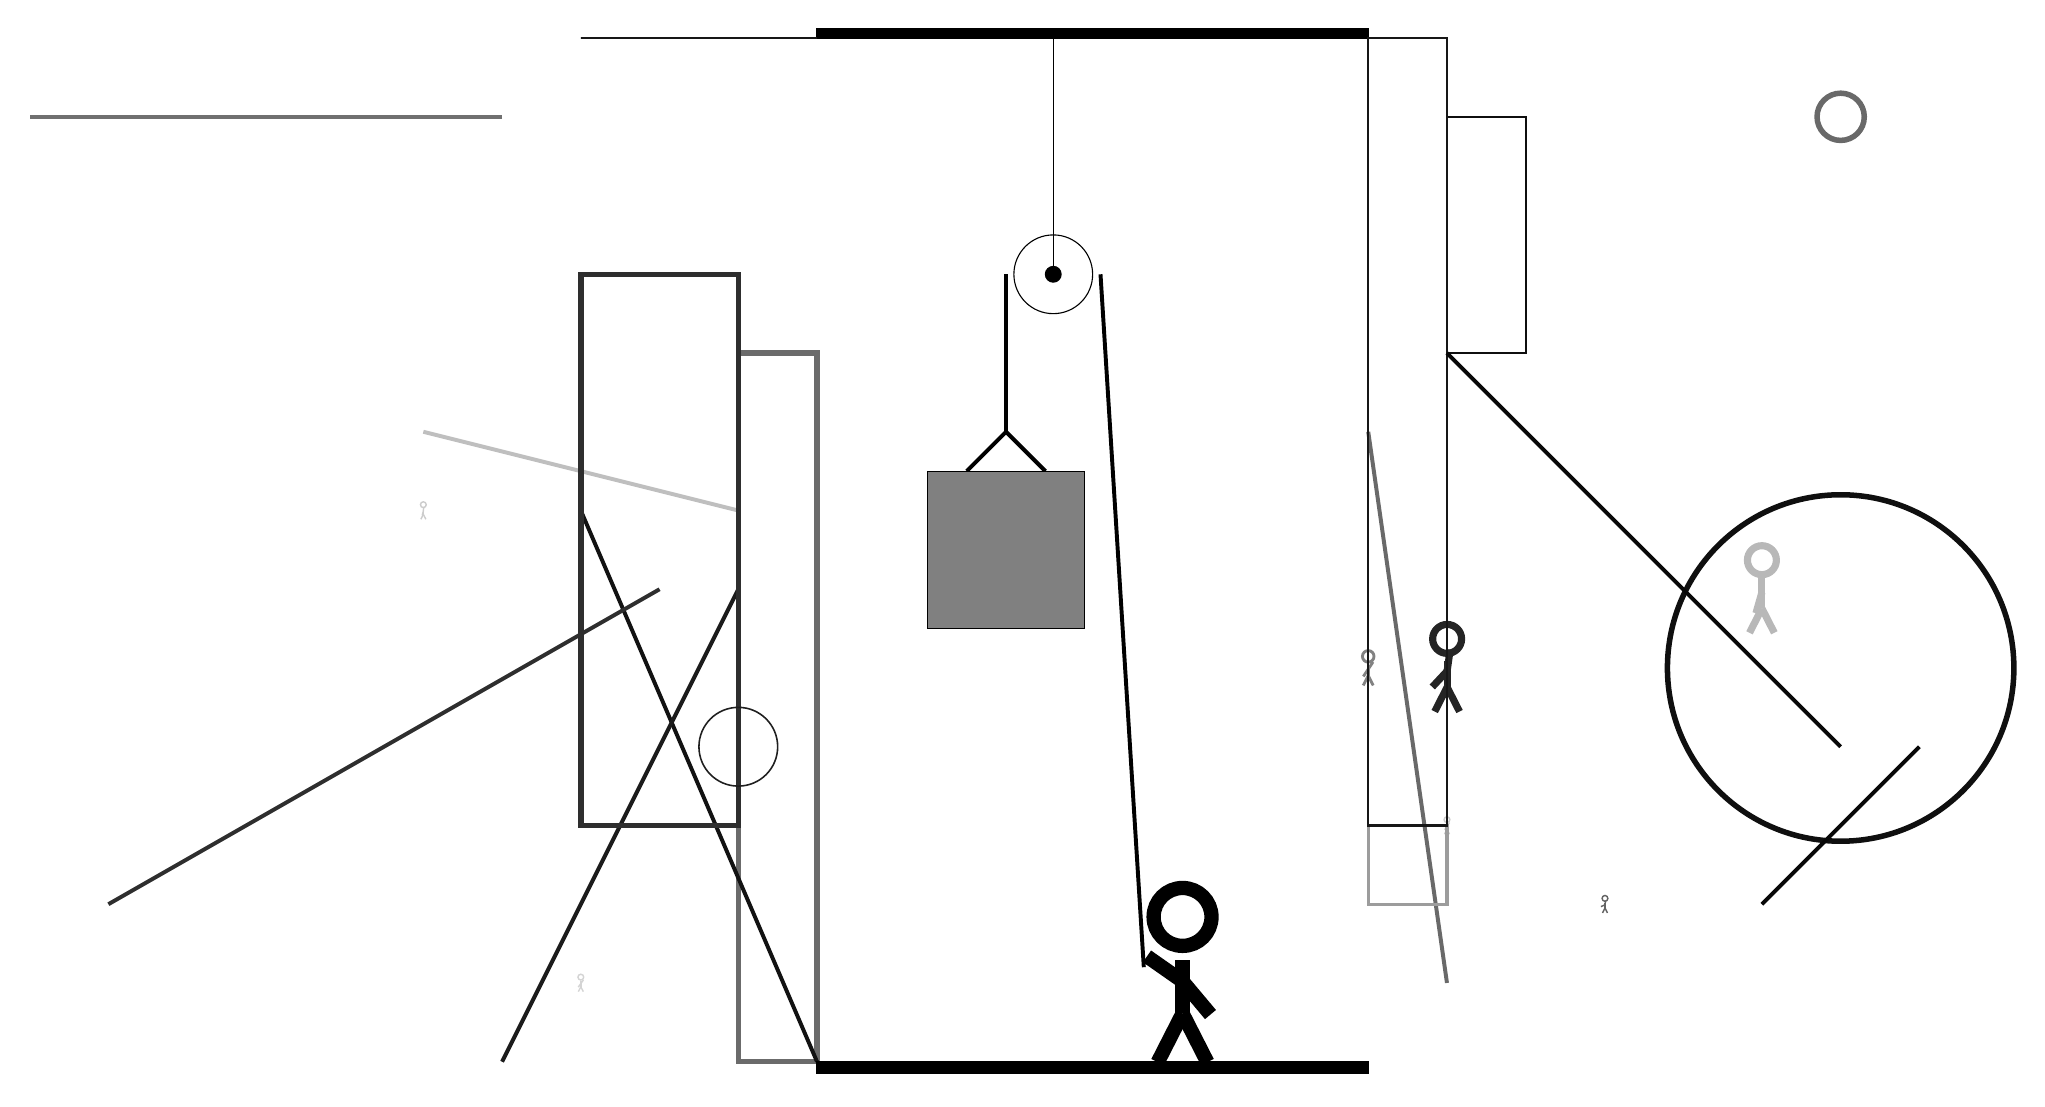
\begin{tikzpicture}
		%%%%% START %%%%%
		
		\draw[fill=black] (-2, 10) rectangle (5, 10.125);
		
		\node[line width=0.4mm, color=black!86] at (6, 2) {\Strichmaxerl[5][47][82]};
		
		\node[line width=0.6mm, color=black!49] at (5, 2) {\Strichmaxerl[2][56][57]};
		\node[line width=0.5mm, color=black!17] at (-5, -2) {\Strichmaxerl[1][54][54]};
		\node[line width=0.3mm, color=black!20] at (6, 0) {\Strichmaxerl[1][60][54]};
		\node[line width=0.5mm, color=black!28] at (10, 3) {\Strichmaxerl[5][74][90]};
		
		\node[line width=0.7mm, color=black!61] at (8, -1) {\Strichmaxerl[1][24][81]};
		\draw[line width=0.5mm, color=black!56](-6, 9) -- (-12, 9);
		\draw[line width=0.5mm, color=black!25](-3, 4) -- (-7, 5);
		\draw[line width=0.5mm, color=black!59](6, -2) -- (5, 5);
		\draw[line width=0.7mm, color=black!58] (-2, -3) rectangle (-3, 6);
		\draw[line width=0.5mm, color=black!93](-2, -3) -- (-5, 4);
		\draw[line width=0.5mm, color=black!89](-3, 3) -- (-6, -3);
		\draw[line width=0.7mm, color=black!82] (-3, 7) rectangle (-5, 0);
		
		\draw[line width=0.3mm, color=black!94] (7, 9) rectangle (6, 6);
		\draw[line width=0.5mm, color=black!82](-4, 3) -- (-11, -1);
		\draw[line width=0.4mm, color=black!39] (5, -1) rectangle (6, 0);
		\draw [line width=0.2mm, color=black!88](-3, 1) circle (0.5);
		
		\draw [line width=0.7mm, color=black!94](11, 2) circle (2.2);
		\draw[line width=0.3mm, color=black!91] (6, 10) rectangle (5, 0);
		
		\draw[line width=0.5mm, color=black!97](6, 6) -- (11, 1);
		\draw [line width=0.5mm, color=black!21](10, -1) circle (0.0);
		
		\node[line width=0.6mm, color=black!20] at (-7, 4) {\Strichmaxerl[1][75][85]};
		
		\draw[line width=0.5mm, color=black!97](10, -1) -- (12, 1);
		\draw[line width=0.3mm, color=black!91] (-2, 10) rectangle (-5, 10);
		\draw [line width=0.7mm, color=black!59](11, 9) circle (0.3);
		
		
		\draw (1, 7) circle (0.5);
		\draw[fill=black] (1, 7) circle (0.1);
		\draw (1, 10) -- (1, 7);
		
		\draw[line width=0.5mm] (-0.1, 4.5) -- (0.4, 5.0) -- (0.9, 4.5);
		\draw[fill=black!50] (-0.6, 4.5) rectangle (1.4, 2.5);
		
		\draw[line width=0.5mm] (0.4, 7) -- (0.4, 5.0);
		\centerarc[line width=0.5mm](1, 7)(0:180:0.6);
		\draw[line width=0.5mm](1.6, 7) -- (2.15, -1.8);
		
		\node at (2.6, -1.9) {\Strichmaxerl[10][-35][-50]};
		
		\draw[fill=black] (-2, -3) rectangle (5, -3.15);
		
		%%%%% END %%%%%
	\end{tikzpicture}
\end{document}